\documentclass[main]{subfiles}

\begin{document}
\setcounter{chapter}{1} %Set chapter counter as week-1
\chapter{More on random walks} %Set chapter name
\setcounter{section}{0}

\lecture{Siva Athreya}{Sanchayan Bhowal, Venkat Trivikram}

\begin{theorem}
    Let $T:\Omega\rightarrow{0,1,\ldots,N}$ be a stopping time. Then,
    $$\E[S_T^2]=E[T].$$
\end{theorem}
\begin{proof}
    $$
        \begin{aligned}
            S_T^2 & =\sum_{k=1}^N S_k^2 \one\{T=k\}                         \\
                  & =\sum_{k=1}^N (S_k^2-S_{k-1}^2) \one\{T\geq k\}         \\
                  & =\sum_{k=1}^N (X_k+S_{k-1})^2-S_{k-1}^2 \one\{T\geq k\} \\
                  & =\sum_{k=1}^N (1+2X_kS_{k-1}) \one\{T\geq k\}.          \\
        \end{aligned}
    $$
    Now, consider $V_k=S_{k-1} \one\{T\geq k\}$. Note that this is a bet sequence. Hence,
    $$
        \begin{aligned}
            \E[S_T^2] & =\E\left[\sum_{k=1}^N\one\{T\geq k\}\right]+2\sum_{k=1}^N\E[X_k V_k] \\
                      & =\sum_{k=1}^N \P(T\geq k)+0                                          \\
                      & =E[T].
        \end{aligned}
    $$
\end{proof}


\section{Reflection Principle}
Assume that $a \in \Z$ and $c>0$. There is a bijection between the paths that cross $a+c$ and those that do not. This bijection is obtained by reflecting the part of the path crossing $a+c$ as shown in the Figure \ref{fig:reflect}. So,
$$\left|S_n=a+c\right|=\left|\sigma_a\leq n \; \& \; S_n=a+c \right|=\left|\sigma_a\leq n \& S_n=a-c \right|$$
Now, we know that all the paths have equal probability. Hence, we get the following lemma.
\begin{lemma}
    $\P(S_n=a+c)=\P(\sigma_a\leq n \; \& \; S_n=a-c)$ where $a \in \Z$ and $c>0$. This is also known as the \emph{reflection principle}.
    \label{lem:reflect}
\end{lemma}
\begin{figure}[ht]
    \label{fig:reflect}
    \centering
    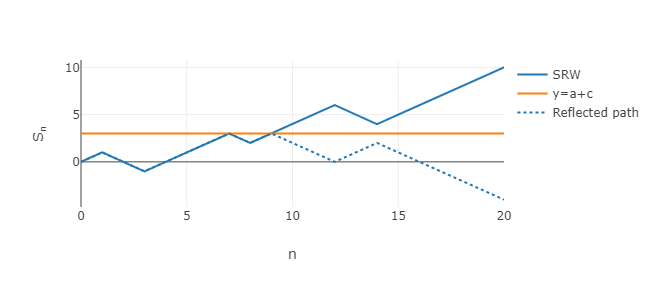
\includegraphics[width=\textwidth]{reflect.png}
    \caption{The figure shows that the bijection between the paths that cross a+c=3 and those that do not.}
\end{figure}
\begin{theorem}
    $\P(\sigma_a\leq n)=\P(S_n\notin [-a,a))$ where $a \in \Z \\ \{0\}$.
\end{theorem}
\begin{proof}
    $$
        \begin{aligned}
            \P(\sigma_a\leq n) & =\P(\sigma_a\leq n, \bigcup_{b \in \Z}{S_n=b} )                                                      \\
                               & =\sum_{b \in \Z} \P(\sigma_a\leq n, S_n=b)                                                           \\
                               & =\sum_{b \in \Z, b\geq a} \P(\sigma_a\leq n, S_n=b)+ \sum_{b \in \Z, b< a} \P(\sigma_a\leq n, S_n=b) \\
                               & =\sum_{b \in \Z, b\geq a} \P(S_n=b)+ \sum_{b \in \Z, b< a} \P(S_n=2a-b)                              \\
                               & =\P(S_n\geq a) + \P(S_n >a)                                                                          \\
                               & =\P(S_n\geq a) + \P(S_n <-a)                                                                         \\
                               & =\P(S_n\notin [-a,a))
        \end{aligned}
    $$
\end{proof}
\begin{corollary}
    $\P(\sigma_a=n)=\frac{1}{2}\left[\P(S_{n-1}=a-1)-\P(S_{n-1}=a+1)\right]$ where $a \in \Z$.
\end{corollary}
\begin{proof}

\end{proof}
\section{Arc-Sine Law}
Let $L$ denote the last time the random walk hits 0, i.e., $L=\max_{0\leq n \leq 2N} {S_n=0},$ where $N$ denotes the length of the walk.
\begin{theorem}
    $$\P(L=2n)=\frac{1}{2^{2N}}\binom{2n}{n}\binom{2N-2n}{N-n}.$$
    \label{thm:arcsin}
\end{theorem}
\begin{remark}
    By Stirling's approximation,
    $$\P(L=2n)\sim \frac{1}{\pi N}\frac{1}{\sqrt{\left(\frac{n}{N}\right)\left(1-\frac{n}{N}\right)}}.$$
    $$
        \begin{aligned}
            \P\left(\frac{L}{2N}\leq x\right) & =\P(L\leq 2Nx)                                                                         \\
                                              & =\sum_{n=0}^{[2Nx]}\P(L=2n)                                                            \\
                                              & \sim \sum_{n=0}^{[2Nx]} \frac{1}{\pi N}\frac{1}{\sqrt{\left(x\right)\left(1-x\right)}} \\
                                              & \sim \int_{0}^{x}\frac{dy}{pi\sqrt{y(1-y)}}                                            \\
                                              & =\frac{2}{\pi}\sin^{-1}(\sqrt{x}).
        \end{aligned}
    $$
\end{remark}
\begin{proof}[Proof of Theorem \ref{thm:arcsin}]
    Define $\tilde{\sigma_0}\inf\{n: S_n=0, 0< n\le N\}$.
    Consider a path of length $2N$ with $L=2n$. This path can be formed by a path which takes $S_2n=0$ and followed by a path of length $2N-2n$ with $\sigma_0>2N-2n$. Hence, number of paths of length $2N$ with $L=2n$ is the product of the number of paths of length $2n$ with $S_{2n}=0$ and the number of paths of length $2N-2n$ with $\sigma_0>2N-2n$.
    Hence,
    \begin{equation}
        \P(L=2n)=\P(S_{2n}=0)\P(\tilde{\sigma_0}>2N-2n),
        \label{eq:distL}
    \end{equation}
    Now let us compute the distribution of $\tilde{\sigma_0}$.
    \begin{equation}
        \begin{aligned}
            \P(\tilde{\sigma_0}>2k) & =\P(S_1\ne 0, \ldots, S_{2k}\ne 0)                                                           \\
                                    & =2\P(S_1> 0, \ldots, S_{2k}> 0)                                                              \\
                                    & =\frac{2}{2^{2k}} \{\text{No. of paths start at 0 and stay above -1 for }2k-1\text{ steps}\} \\
                                    & =\frac{2}{2^{2k}} \{\text{No. of paths start at 0 and stay below 1 for }2k-1\text{ steps}\}  \\
                                    & =\P(\sigma_1>2k-1)                                                                           \\
                                    & =1-\P(\sigma_1\geq 2k-1)                                                                     \\
                                    & =\P(S_{2k-1}=-1)+\P(S_{2k-1}=0)                                                              \\
                                    & =\P(S_{2k-1}=-1)
        \end{aligned}
        \label{eq:tilds}
    \end{equation}
    Using \eqref{eq:distL} and \eqref{eq:tilds},
    $$
        \begin{aligned}
            \P(L=2n) & =\P(S_{2n}=0)\P(S_{2N-2n-1}=-1)                    \\
                     & =\P(S_{2n}=0)\P(S_{2N-2n}=0)                       \\
                     & = \frac{1}{2^{2N}}\binom{2n}{n}\binom{2N-2n}{N-n}.
        \end{aligned}
    $$
    The first step analysis of $S_{2n}$ shows that, $\P(S_{2N-2n}=0)=\frac{1}{2}\P(S_{2N-2n-1}=1)+\frac{1}{2}\P(S_{2N-2n-1}=-1)$. Using the symmetry of the walk we know that $\P(S_{2N-2n-1}=1)=\P(S_{2N-2n-1}=-1)$. This gives the second inequality.
\end{proof}


\section{SRW of length $N$ in $\Z^d$}
\subsection{Notations and notions in higher dimension}
\begin{itemize}
    \item $e_i \in \Z^d,\, \forall\,i \in \{1,2,\cdots,d\}$, defined as the vector of length $d$ with all entries zeroes except $i^{th}$ being 1.
          $$e_i = (0,0,\cdots,\underbrace{1}_{i^{th}},0,\cdots,0)$$
    \item For $x \in \Z^d,$
          $$\,x = \sum\limits_{i=1}^{d}x_{i}e_{i},\,x_i \in \Z\hspace{1.5cm}\lVert x \rVert = \left(\sum\limits_{i=1}^{d}x_{i}^{2}\right)^{\frac{1}{2}}$$
    \item $\Omega_N = \{(\omega_1,\omega_2,\cdots,\omega_N) \mid \omega_i \in \Z^d, \lVert \omega_i \rVert  = 1\,\forall\,1 \leq i \leq N\}$
    \item We have, for $1\leq k,n \leq N$ $$X_k : \Omega_N \to \Z^d,\,X_{k}(\omega) = \omega_k \hspace{1.5cm} S_n : \Omega_N \to \Z^d,\,S_n(\omega) = \sum\limits_{k=1}^n X_k(\omega)$$
          with $ S_{0}(\omega)=0 $. We can consider $S_n$ as a $d$-dimensional vector given by $S_n = \left(S_n^{(1)},S_n^{(2)},\cdots S_n^{(d)}\right)$, where each $S_n^{(i)}$ is a random walk on $\Z$.
    \item The probability function $\P^N$, given by,
          $$ \P^N : \mathcal{P}(\Omega_N) \to [0,1],\,\,\,\,\,\,\,\P(A) = \frac{|A|}{(2d)^N}\,\forall\,A \subseteq \Omega_N$$
\end{itemize}
\subsection{Infinite length random walk}
On extending $N \to \infty$, we preserve something called as ``consistency". First, let us define, for $0<N<M$,
$$\pi_N : \Omega_M \to \Omega_N,\,\,\,\pi_N(\omega_1,\omega_2,\cdots,\omega_M) = (\omega_1,\omega_2,\cdots,\omega_N)$$

Under $(\Omega_N,\mathcal{P}(\Omega_N),\P^N)$ and $(\Omega_M,\mathcal{P}(\Omega_M),\P^M)$, if we observe the walk till time $n < N$ the probability of evenets concerning the walk should be same under $\P^N$ or $\P^M$. For any event $\{\tilde{\omega} \in \Omega_N\}$, there exists a corresponding same event namely $\{\omega \in \Omega_M : \pi_N(\omega) = \tilde{\omega}\}.$ We have,
$$\P^N(\{\tilde{\omega}\}) = \frac{1}{(2d)^N} \hspace{2cm} \P^M(\{\omega \in \Omega_M : \pi_N(\omega) = \tilde{\omega}\}) = \frac{(2d)^{M-N}}{(2d)^M} = \frac{1}{(2d)^N}$$

So, we say the sequence of probability spaces $(\Omega_1,\P^1),(\Omega_2,\P^2),\cdots,(\Omega_N,\P^N)$ satisfies the consistency condition
$$\P^N(\{\tilde{\omega}\}) = \frac{1}{(2d)^N} = \frac{(2d)^{M-N}}{(2d)^M}=\P^M(\{\omega \in \Omega_M : \pi_N(\omega) = \tilde{\omega}\}),\,0<N<M,\,\tilde{\omega} \in \Omega_N $$

We define the space of infinite sequences,
$$\Omega_{\infty} = \{\omega = (\omega_k)k \geq 1 \mid \omega_k \in \Z^d,\,\lVert \omega_k \rVert = 1\}$$
$$\mathcal{A}_{\infty}\,(\equiv \mathcal{P}(\Omega_{\infty}))\,\text{denotes the class of events observable ``for ever"}$$

For $N \in \N$,
$$\pi_N : \Omega_{\infty} \to \Omega_N,\,\,\,\pi_N(\omega) = (\omega_1,\omega_2,\cdots,\omega_N)$$

\begin{theorem}[\textbf{Kolmogorov Consistency Theorem}]
    \normalfont
    There exists a unique probability measure on $(\Omega_{\infty},\mathcal{A}_{\infty})$ such that $\forall\,N \geq 1,\,\forall\,\tilde{\omega} \in \Omega_N$,
    $$\P^N(\{\tilde{\omega}\}) =\P^M(\{\omega \in \Omega_M : \pi_N(\omega) = \tilde{\omega}\})= \frac{1}{(2d)^N}$$
\end{theorem}
Now, we can define,
$$X_k : \Omega_{\infty} \to \Z^d,\,\,X_k(\omega) = \omega_k \hspace{2cm} S_n = \sum_{k=1}^{n} X_k\,\,\forall\,n \geq 1$$

under $\P$, $\{S_n\}_{n \geq 1}$ is a simple random walk starting at $S_0 = 0$.

\begin{definition}
    \normalfont
    $A \subseteq \Omega_{\infty}$ is said to be \textbf{observable} by time $ n $ if $A$ is a union of the events of the form
    $$\{\omega \in \Omega_{\infty} : \omega_i = o_i,\,1 \leq i \leq N\}\,\,\text{with}\,\,o_i \in \Z^d,\,\lVert o_i \rVert = 1$$
\end{definition}

For, $k \in \N_{0}$, $\mathcal{A}_k$ denotes the set of all events in $\Omega_{\infty}$ observable by time $k$.

\begin{definition}
    \normalfont
    $T : \Omega_{\infty} \to \N \cup \{\infty\} \cup \{0\}$ is a \textbf{stopping time} if
    $$\text{for any}\,\,\,k \in \N_{0},\,\{T=k\} \in \mathcal{A}_k$$
\end{definition}

For example, $\sigma_a = \min\{n \geq 0 \mid S_n = a\}$ is a stopping time.
\subsection{Speed of the walk}
\begin{definition}
    \normalfont
    For, $S_n = \sum\limits_{k=1}^{n}X_k$, we define \textbf{speed of the walk} as $$\text{Speed}\,\,=\,\, \frac{S_n}{n}=\frac{1}{n}\sum\limits_{k=1}^{n}X_k$$
\end{definition}

We have, $X_k = \left(X_k^{(1)},X_k^{(2)},\cdots,X_k^{(d)}\right)$, $\{X_k\}_{k \geq 1}$ which is an i.i.d sequence of random variables with
$$\P(X_k = e_i) = \frac{1}{2d} = \P(X_k = -e_i)$$
$\Rightarrow\,\E[X_k] = 0$ and $\E[\lVert X_k \rVert] = 1\,\,(\leq \infty)$

\begin{theorem}[\textbf{Strong law of large numbers}]
    \normalfont
    For simple random walk on $\Z^d$,
    $$\frac{S_n}{n} \rightarrow 0\,\,\text{with probability}\,\,1\,\,\text{under}\,\,(\Omega_{\infty},\mathcal{A}_{\infty},\P)$$
\end{theorem}

\subsection{Typical position of the walk}
For $d=1$,

\begin{align*}
    \frac{S_n - (n)(0)}{\sqrt{n}} \xrightarrow{\,\,\,\,d\,\,\,\,\,} \mathcal{N}(0,1) \\
    \Rightarrow	\,\,\, \sqrt{n}\left(\frac{S_n}{n}\right)  \xrightarrow{\,\,\,\,d\,\,\,\,\,}  \mathcal{N}(0,1)
\end{align*}
For $d >1$, $\mu \in \mathbb{R}^d$ and a positive definite matrix $\Sigma \in \mathbb{R}^{d \times d}$, we have $d$-dimensional normal distribution as,
$$\Phi_{d,\mu,\Sigma}(y) = \frac{1}{(2 \pi)^{d/2}} \frac{1}{\det(\Sigma)^{1/2}} \exp \left(-\frac{1}{2}(x-\mu)^{t} \Sigma^{-1} (x- \mu)\right)$$

$$\P \left(\frac{S_n}{\sqrt{n}}\in \prod\limits_{i=1}^{d} [a_i,b_i] \right)  \xrightarrow[n \to \infty]{}  \int\limits_{\prod\limits_{i=1}^{d} [a_i,b_i]} \Phi_{d,0,\Sigma^d}(y) \,dy$$
where, $\mu =0,\,
    \Sigma^d =  \text{diag}\,(\frac{1}{d},\cdots,\frac{1}{d})$
\subsection{Large deviation principle}
From the CLT, we have that
$$\P(\lVert S_n \rVert > a\sqrt{n}) \xrightarrow[n \to \infty]{} \int\limits_{\lVert x \rVert >a} \Phi_{d,0,\Sigma^d}(y) \,dy$$

We consider the events of the form $\{\lVert S_n \rVert > an\},\,a\in [0,\infty)$, which are ``rare" in the sense that their probabiility tends to 0 as $n \to \infty$. On formal application of CLT shows that probability of these rare events are exponentially small.
\begin{theorem}[\textbf{Cramer's theorem}]
    \normalfont
    For, $a>0$,
    $$\lim\limits_{n \to \infty} \frac{\log(\P(\lVert S_n \rVert > an))}{n} = -I(a)$$

    where,
    $$
        I(a) =
        \begin{cases}
            \log2 + \frac{1+a}{2}\log \frac{1+a}{2} + \frac{1-a}{2} \log\frac{1-a}{2}, & \text{for}\,\,a \in [-1,1] \\
            \infty,                                                                    & \text{otherwise}
        \end{cases}
    $$

    It can be vaguely interpreted as, $\P(\lVert S_n \rVert > na) \sim e^{-nI(a)}$
\end{theorem}

\section{Exercises}
\begin{enumerate}
    \item Complete the proof of Reflection Principle (Lemma \ref{lem:reflect}).
    \item Find the distribution of $M_k=\max_{1\leq k\leq n} S_k$.
    \item Show that $\E[\lVert X_k \rVert] = 1$.
\end{enumerate}
\end{document}